\chapter{Hardware and Software Selection}
\label{sec:HardwareSoftwareSelection}

Building upon insights from the previous chapters and the integral role of haptic feedback in enhancing user experience, this section delineates the specific hardware components and software solutions capable of delivering sophisticated haptic feedback for keyboard typing in virtual environments.

\section{Head-mounted Devices}
\label{sec:HeadMountedDevices}

In our investigation, the Meta Quest 3 is selected as the primary head-mounted display (HMD) due to its superior features when compared to its predecessors and competitors. This decision follows a comprehensive analysis of its capabilities in contrast to the HTC Vive and Oculus Rift.

\begin{itemize}
    \item \textbf{Meta Quest 3} offers a high-resolution LCD (2064x2208 per eye), a 120Hz refresh rate, and advanced tracking capabilities including 6 degrees of freedom (DoF) inside-out tracking via 4 integrated cameras and a depth sensor. It supports hand tracking and includes two 6DoF Meta Quest Touch Plus Controllers, providing robust connectivity options such as WiFi streaming, WiFi 6E, and Bluetooth.
    
    \item \textbf{HTC Vive}, on the other hand, features an OLED display with a resolution of 1080x1200 per eye and a 90Hz refresh rate. It employs a marker-based tracking system and includes two 6DoF HTC Vive controllers but lacks hand tracking, WiFi, and Bluetooth.
    
    \item \textbf{Oculus Rift} provides an AMOLED display with a resolution of 1080x1200 per eye and a 90Hz refresh rate. It uses an outside-in tracking system and includes two first-generation 6DoF Oculus Touch controllers but does not support hand tracking, WiFi, or Bluetooth.
\end{itemize}
Given these specifications, Meta Quest 3 is chosen for its cutting-edge display quality, superior tracking, and enhanced connectivity, making it the most suitable option for our experiments.

\section{Haptic Sensations and Devices}
\label{sec:HapticSensationsDevices}

The role of haptic devices in virtual reality is to bridge the gap between the real and virtual worlds by transmitting tactile sensations. A company named SynTouch has developed a product known as the SynTouch-Toccare Haptics Measurement System, capable of quantifying 15 haptic dimensions of any material, thus replicating human touch perception. This technology is pivotal in providing a nuanced understanding of material textures and interactions within the virtual environment.
\begin{figure}[ht]
  \centering
  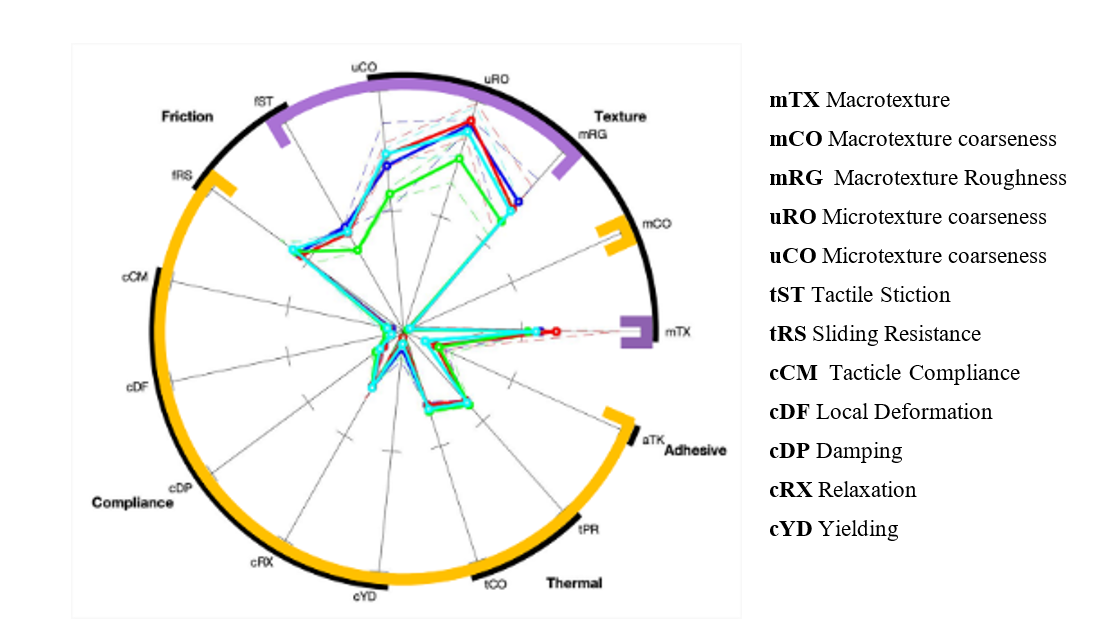
\includegraphics[width=0.8\textwidth]{Development/senstations.PNG}
  \caption{SynTouch's 15-Dimensional Sensations \cite{quantifying_touch}}
  \label{fig:sensations}
\end{figure}

\subsection{Advanced Haptic Gloves}
\label{subsec:AdvancedHapticGloves}

For the experimental setup, we propose using the SenseGlove Nova, renowned for its advanced haptic feedback capabilities and innovative design. The SenseGlove Nova offers a range of features that enhance the realism and immersion of virtual reality interactions:

\begin{figure}[ht]
\centering
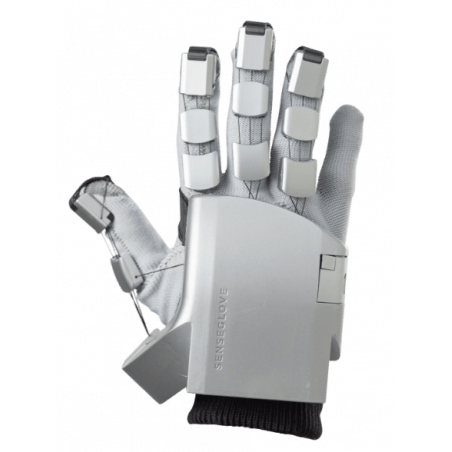
\includegraphics[width=0.35\textwidth]{Development/sense-glove-nova-set.jpg}
\caption{The Sense Glove Nova \cite{senseglove_nova}}
\label{fig: The Sense Glove Nova}
\end{figure}

\begin{itemize}
\item \textbf{Force Feedback:} Each glove is equipped with high-precision brakes that deliver up to 20N of force on each finger. This feature enables users to feel the weight and resistance of virtual objects, ranging from heavy tools to delicate items, providing a more authentic interaction experience \cite{senseglove_nova}.
\item \textbf{Vibrotactile Feedback:} The SenseGlove Nova incorporates vibrotactile actuators that generate realistic sensations such as button clicks, vibrations, and impacts. This feedback significantly enhances the user's sense of touch and engagement with virtual environments \cite{vibrotactile_feedback}.

\item \textbf{Sensor-Based Tracking:} The gloves utilize multiple high-accuracy sensors to capture the movements of the thumb and fingers. This precise tracking is crucial for accurate hand representation in virtual reality, ensuring that user actions are mirrored accurately within the virtual space \cite{sensor_tracking}.
\end{itemize}
\noindent
The SenseGlove Nova's combination of force feedback, vibrotactile feedback, and precise tracking makes it an ideal choice for applications requiring detailed and nuanced hand interactions. Its advanced technology supports a wide range of virtual reality applications, from training simulations to interactive gaming, by providing users with a tactile experience that closely mimics real-world interactions.\\ \\
The use of SenseGlove Nova in our experimental setup is expected to significantly enhance the user experience by providing realistic and responsive haptic feedback. This technology not only improves the immersion but also aids in tasks requiring fine motor skills and detailed manipulation of virtual objects, making it a valuable tool for our virtual reality system \cite{advanced_haptic_gloves_review}.

\section{Virtual Environment Development with Unity}
\label{subsec:VirtualEnvironmentDevelopmentWithUnity}

Unity will be utilized for developing the virtual environment in which the virtual keyboard will be used. The advantages of using Unity include:
\begin{itemize}
\item \textbf{Real-Time Rendering:} Unity's powerful real-time rendering capabilities ensure smooth and immersive visuals, essential for creating a realistic virtual environment.
\item \textbf{Cross-Platform Support:} Unity supports multiple platforms, allowing the virtual environment to be accessible on various devices, from VR headsets to mobile devices and PCs.
\item \textbf{Extensive Asset Store:} Unity's Asset Store provides a vast array of pre-made assets, scripts, and plugins that can accelerate development and add rich features to the environment.
\item \textbf{Robust Developer Community:} A large and active community of developers means extensive support, tutorials, and forums for problem-solving and learning.
\item \textbf{Seamless Integration with Other Tools:} Unity can easily integrate with other development tools and software, facilitating a cohesive and efficient development process.
\end{itemize}
Using Unity ensures that our virtual environment will be engaging, versatile, and accessible, providing users with a seamless and immersive experience while interacting with the virtual keyboard.


\section{Keyboard Design with Blender}
\label{subsec:KeyboardDesignWithBlender}

For the design and modeling of the virtual keyboard, we will use Blender, a powerful and versatile 3D modeling software. Blender is chosen for several reasons:
\begin{itemize}
\item \textbf{Comprehensive Toolset:} Blender offers an extensive range of tools for modeling, sculpting, texturing, and rendering, making it an all-in-one solution for creating detailed and high-quality 3D models.
\item \textbf{Open Source and Free:} Blender is open-source software, which means it is free to use. This allows us to allocate resources to other aspects of the project while still utilizing professional-grade software.
\item \textbf{Community Support and Documentation:} Blender has a large, active community and extensive documentation, providing ample resources for troubleshooting and learning advanced techniques.
\item \textbf{Integration Capabilities:} Blender supports various file formats and can be integrated with other software tools used in our project, ensuring a smooth workflow.
\end{itemize}
Using Blender allows us to create a highly detailed and customizable virtual keyboard, enhancing the user's interaction experience by providing a visually appealing and functional design.

\section{Integration With Meta Quest 3}
\label{subsec:IntegrationWithMetaQuest3}

The integration of SenseGlove Nova with the Meta Quest 3 is facilitated through the SenseGlove Nova SDK \cite{senseglove_sdk} . Connections can be established via Bluetooth or by directly linking the glove's controller transform object into the virtual environment setup. This integration allows for precise control over force feedback and tactile sensations, ensuring a rich and immersive user experience.





\section{Assisting and Guiding}
\label{sec:AssistingGuiding}

In addition to enhancing the surrounding area of the virtual keyboard to assist users during typing by providing directions and guidelines, we will integrate advanced language understanding features through a third-party service called ChatGPT. This integration aims to improve the structure and content of entered text by offering sentence and word suggestions \cite{openai, ioshacker}. Users will be able to select the most suitable suggestion for their attention, thus elevating the overall typing experience. ChatGPT, trained on a diverse range of internet text, possesses advanced language understanding capabilities, enabling it to generate human-like text based on provided context \cite{openai}. This unique attribute makes it an ideal tool for suggesting contextually relevant and grammatically correct words or sentences, surpassing the capabilities of simple auto-correct systems. Unlike traditional auto-correct systems that focus solely on the last word typed, ChatGPT provides contextual suggestions by considering the overall context of the sentence \cite{yellow, online-tech}. This approach results in more accurate and helpful suggestions, contributing to an improved user experience. \\ \\
The integration of ChatGPT goes beyond correcting typos; it enriches the typing experience by allowing users to explore different ways to express their thoughts with the assistance of versatile suggestions. This not only enhances efficiency but also adds an element of enjoyment to the typing process \cite{ioshacker}. Furthermore, ChatGPT's continuous learning capability as a machine learning model means that it can improve over time. The more it is utilized, the better it becomes at providing relevant suggestions, ensuring a dynamic and evolving tool for users. In terms of versatility, ChatGPT can be seamlessly adapted to various applications, making it a valuable tool in diverse scenarios beyond typing assistance. Its versatility extends its utility across different domains, showcasing its potential as a multifaceted solution \cite{openai}.



\section{Summary}
\label{sec:Summary}

Selecting appropriate hardware and software is crucial for achieving a high-fidelity virtual experience. The chosen devices support advanced delivery of haptic feedback and ensure a seamless, intuitive user experience. By integrating these technologies, we aim to create a virtual typing interface that closely mimics real-world interactions, thereby enhancing realism and effectiveness in the virtual environment.
